\documentclass[12pt,fleqn]{article}\usepackage{../../common}
\begin{document}
�ift Sarka� (Double Pendulum)

En basit formunda �ifte sarka� $l$ uzunlu�unda k�tlesiz iki �ubuk, iki $m$
k�tlesindeki topu birle�tirir, yani $m_1=m_2=m$, ve salland�r�r. E�er
$m_1$'in oldu�u kordinatlar� $x_1,y_1$, $m_2$ k�tlesini $x_2,y_2$ ile
belirtirsek,

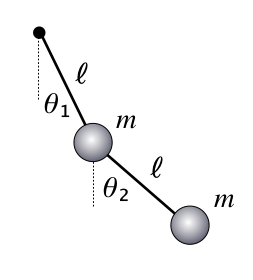
\includegraphics[width=15em]{phy_dblpend_01.png}

$$
x_1 = \ell \sin\theta_1, \quad y_1 = - \ell \cos\theta_1
$$

$$
x_2 = \ell  (\sin\theta_1 +  \sin\theta_2) , \quad 
y_2 = -\ell  (\cos\theta_1 + \cos \theta_2)
$$






\begin{minted}[fontsize=\footnotesize]{python}
import math, pylab
import numpy as np
from matplotlib.patches import Circle
import matplotlib.pyplot as plt

g = 9.8 # standard freefall (m/s^2)

l = 1
L1 = 1
L2 = 1
theta10 = 3*np.pi/7
theta20 = 3*np.pi/4
dt = 0.01
tmax = 10

nsteps = int(tmax/dt)
t = [0.0]*nsteps
p1 = [0.0]*nsteps
p2 = [0.0]*nsteps
q1 = [0.0]*nsteps
q2 = [0.0]*nsteps
x1 = [0.0]*nsteps
x2 = [0.0]*nsteps
y1 = [0.0]*nsteps
y2 = [0.0]*nsteps

# initialize
q1[0] = theta10                              
q2[0] = theta20                              
x1[0] = l*math.sin(q1[0])                    
y1[0] = - l*math.cos(q1[0])                  
x2[0] = l*(math.sin(q1[0])+math.sin(q2[0]))  
y2[0] = - l*(math.cos(q1[0])+math.cos(q2[0]))

# use Euler-Cromer method to integrate the double pendulum
for i in range(nsteps - 1):
    s = math.sin(q1[i] - q2[i])                               
    c = math.cos(q1[i] - q2[i])                               
    D = l**2*(1+s**2)                                         
    A = p1[i]*p2[i]*s/D                                       
    B = (p1[i]**2+2*p2[i]**2 - 2*p1[i]*p2[i]*c)*s*c*l**2/D**2 

    p1[i+1] = p1[i] - (2*g*l*math.sin(q1[i]) - A+B)*dt
    p2[i+1] = p2[i] - (g*l*math.sin(q2[i])+A - B)*dt
    q1[i+1] = q1[i]+(p1[i+1] - p2[i+1]*c)/D*dt
    q2[i+1] = q2[i]+(2*p2[i+1] - p1[i+1]*c)/D*dt
    t[i+1] = t[i]+dt

    # put q1 and q2 in range -pi to +pi
    q1[i+1] = (q1[i+1]+math.pi)%(2.0*math.pi) - math.pi
    q2[i+1] = (q2[i+1]+math.pi)%(2.0*math.pi) - math.pi
    
    # also compute (x,y) locations of points 1 and 2
    x1[i+1] = l*math.sin(q1[i+1])                       
    y1[i+1] = - l*math.cos(q1[i+1])                     
    x2[i+1] = l*(math.sin(q1[i+1])+math.sin(q2[i+1]))   
    y2[i+1] = -  l*(math.cos(q1[i+1])+math.cos(q2[i+1]))

# Plotted bob circle radius
r = 0.05
# Plot a trail of the m2 bob's position for the last trail_secs seconds.
trail_secs = 0
# This corresponds to max_trail time points.
max_trail = int(trail_secs / dt)

def make_plot(i):
    # Plot and save an image of the double pendulum configuration for time
    # point i.
    # The pendulum rods.
    ax.plot([0, x1[i], x2[i]], [0, y1[i], y2[i]], lw=2, c='k')
    # Circles representing the anchor point of rod 1, and bobs 1 and 2.
    c0 = Circle((0, 0), r/2, fc='k', zorder=10)
    c1 = Circle((x1[i], y1[i]), r, fc='b', ec='b', zorder=10)
    c2 = Circle((x2[i], y2[i]), r, fc='r', ec='r', zorder=10)
    ax.add_patch(c0)
    ax.add_patch(c1)
    ax.add_patch(c2)

    # The trail will be divided into ns segments and plotted as a fading line.
    ns = 20
    s = max_trail // ns

    for j in range(ns):
        imin = i - (ns-j)*s
        if imin < 0:
            continue
        imax = imin + s + 1
        # The fading looks better if we square the fractional length along the
        # trail.
        alpha = (j/ns)**2
        ax.plot(x2[imin:imax], y2[imin:imax], c='r', solid_capstyle='butt',
                lw=2, alpha=alpha)

    # Centre the image on the fixed anchor point, and ensure the axes are equal
    ax.set_xlim(-L1-L2-r, L1+L2+r)
    ax.set_ylim(-L1-L2-r, L1+L2+r)
    ax.set_aspect('equal', adjustable='box')
    plt.axis('off')
    plt.savefig('/home/burak/Downloads/frames/img{:04d}.png'.format(i), dpi=72)
    plt.cla()

    
fps = 10
di = int(1/fps/dt)
fig = plt.figure(figsize=(8.3333, 6.25), dpi=72)
ax = fig.add_subplot(111)
tmax, dt = 30, 0.01
t = np.arange(0, tmax+dt, dt)
for i in range(0, t.size, di):
    if i==1000: break
    if i % 20 == 0:
        print (i)
        make_plot(i)
\end{minted}


\begin{minted}[fontsize=\footnotesize]{python}
! convert -loop 0 -delay 100 frames/*.png frames/dblpend.gif
\end{minted}








Kaynaklar

[1] Creighton, {\em Numerical Methods}

[2] Bayramli, {\em Double Pendulum Animasyonu}, \url{https://github.com/burakbayramli/classnotes/blob/master/phy/phy_dblpend/frames/dblpend.gif}

\end{document}

